\tasknumber{2018}{7} Решить уравнение $|x-7|+|x-5|=x-4$\\
Построим на числовой оси знаки раскрытия модулей в зависимости от $x$\\
\begin{center}
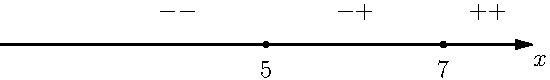
\includegraphics[scale =1]{7.pdf}\\
1 случай $x\leqslant5$\\
$-x+7-x+5=x-4 \Leftrightarrow -3x=-16\Leftrightarrow x=\frac{16}3$\\
$\frac{16}3>5 \Rightarrow x=\frac{16}3 - \text{не подходит.}$\\
2 случай $5<x<7$\\
$-x+7+x-5=x-4 \Leftrightarrow x=6$\\
$5<6<7 \Rightarrow x=6 - \text{походит.}$\\
3 случай $x\geqslant 7$\\
$x-7+x-5=x-4 \Leftrightarrow x=8$\\
$8\geqslant7 \Rightarrow x=8 - \text{подходит.}$\\
\end{center}
\Answer{\{6;8\}}
